\documentclass{article}

% content/resources/templates/preamble.tex
\usepackage[margin=0.6in]{geometry}
\author{Milav Dabgar}
\usepackage{amsmath,amssymb,amsthm}
\usepackage{booktabs}
\usepackage{multirow}
\usepackage{xcolor}
\usepackage{tcolorbox}
\tcbuselibrary{breakable,skins}
\usepackage[colorlinks=true,linkcolor=blue]{hyperref}
\usepackage{titlesec}
\usepackage{enumitem}
\usepackage{tikz}
\usepackage{pgfplots}
\usepackage{circuitikz}
\usepackage[version=4]{mhchem}
\usepackage{longtable}
\usepackage{array}
\usepackage{float}
\usepackage{caption}
\usepackage{listings}

\lstset{
  basicstyle=\small\ttfamily,
  breaklines=true,
  breakatwhitespace=false,
  postbreak=\mbox{\textcolor{red}{$\hookrightarrow$}\space},
  float=false,
  numbers=left,
  numberstyle=\tiny\color{gray},
  numbersep=10pt,
  xleftmargin=2em,
  keywordstyle=\color{blue},
  commentstyle=\color{green!60!black},
  stringstyle=\color{purple},
  backgroundcolor=\color{gray!5},
  showstringspaces=false,
  tabsize=2,
  captionpos=b,
  keepspaces=true,
  columns=flexible
}

\pgfplotsset{compat=1.18}
\usetikzlibrary{shapes,arrows,positioning,calc,patterns,decorations.pathmorphing,decorations.markings,arrows.meta}

% Color scheme
\definecolor{headcolor}{RGB}{0,102,204}
\definecolor{keycolor}{RGB}{220,20,60}
\definecolor{solutioncolor}{RGB}{34,139,34}
\definecolor{mnemoniccolor}{RGB}{148,0,211}
\definecolor{codecolor}{RGB}{0,0,100}

% Spacing
\setlength{\parskip}{3pt}
\setlist[itemize]{nosep}
\setlist[enumerate]{nosep}

% Title formatting
\titleformat{\section}{\Large\bfseries\color{headcolor}}{\thesection}{1em}{}
\titleformat{\subsection}{\large\bfseries\color{headcolor}}{\thesubsection}{1em}{}

% Pandoc tightlist compatibility
\providecommand{\tightlist}{%
  \setlength{\itemsep}{0pt}\setlength{\parskip}{0pt}}

% Pandoc longtable compatibility
\newcounter{none}
\def\thenone{}


% content/resources/templates/english-boxes.tex

% Custom environments
\newtcolorbox{solutionbox}{
 breakable,
 enhanced,
 colback=solutioncolor!5!white,
 colframe=solutioncolor!75!black,
 fonttitle=\bfseries,
 title=Solution
}

\newtcolorbox{solutionboxnobreak}{
 colback=solutioncolor!5!white,
 colframe=solutioncolor!75!black,
 fonttitle=\bfseries,
 title=Solution
}

\newtcolorbox{keyformula}{
 breakable,
 enhanced,
 colback=keycolor!5!white,
 colframe=keycolor!75!black,
 fonttitle=\bfseries,
 title=Key Formula
}

\newtcolorbox{mnemonicboxenv}{
 breakable,
 enhanced,
 colback=mnemoniccolor!5!white,
 colframe=mnemoniccolor!75!black,
 fonttitle=\bfseries,
 title=Mnemonic
}

\newcommand{\mnemonicbox}[1]{%
  \begin{mnemonicboxenv}
    #1
  \end{mnemonicboxenv}
}


% Custom commands for GTU solutions
% This file defines semantic commands for consistent formatting

% Question command with automatic formatting
\newcommand{\question}[2]{%
  \section*{Question #1}%
  \textbf{#2}%
}

% OR question variant
\newcommand{\questionor}[2]{%
  \section*{Question #1 OR}%
  \textbf{#2}%
}

% Proper table environment with caption
\newenvironment{answertable}[1]{%
  \begin{table}[htbp]
  \centering
  \caption{#1}
}{%
  \end{table}
}

% Proper figure environment for diagrams
\newenvironment{answerdiagram}[1]{%
  \begin{figure}[htbp]
  \centering
  \caption{#1}
}{%
  \end{figure}
}

% Semantic markup for key terms
\newcommand{\keyword}[1]{\textbf{#1}}
\newcommand{\code}[1]{\texttt{#1}}
\newcommand{\classname}[1]{\texttt{#1}}
\newcommand{\methodname}[1]{\texttt{#1}}

% Proper quotation marks
\newcommand{\mnemonic}[1]{``#1''}


\title{Introduction to IT Systems (4311602) - Winter 2023 Solution}
\date{January 18, 2024}

\begin{document}
\maketitle

\questionmarks{1(a)}{3}{Differentiate between Information and Knowledge.}

\begin{solutionbox}
\textbf{Answer:}

\begin{answertable}{Information vs Knowledge}
\begin{tabulary}{\linewidth}{|L|L|L|}
\hline
\textbf{Aspect} & \textbf{Information} & \textbf{Knowledge} \\
\hline
\textbf{Definition} & Raw facts and figures & Processed information with understanding \\
\hline
\textbf{Processing} & Data that is organized & Information combined with experience \\
\hline
\textbf{Application} & Can be shared easily & Requires interpretation and context \\
\hline
\end{tabulary}
\end{answertable}

\begin{itemize}
    \item \keyword{Information}: Raw facts, data, and figures that can be processed
    \item \keyword{Knowledge}: Understanding gained through experience and learning
\end{itemize}

\begin{mnemonicbox}
\mnemonic{Information Informs, Knowledge Knows}
\end{mnemonicbox}
\end{solutionbox}

\questionmarks{1(b)}{4}{Explain Functions of OS.}

\begin{solutionbox}
\textbf{Answer:}

\textbf{Primary Functions of Operating System:}

\begin{answertable}{OS Functions}
\begin{tabulary}{\linewidth}{|L|L|}
\hline
\textbf{Function} & \textbf{Description} \\
\hline
\textbf{Process Management} & Controls execution of programs \\
\hline
\textbf{Memory Management} & Allocates and deallocates memory \\
\hline
\textbf{File Management} & Organizes and manages files \\
\hline
\textbf{Device Management} & Controls input/output devices \\
\hline
\end{tabulary}
\end{answertable}

\begin{itemize}
    \item \textbf{Process Control}: Scheduling and managing running programs
    \item \textbf{Resource Allocation}: Distributing system resources efficiently
    \item \textbf{User Interface}: Providing interaction between user and computer
\end{itemize}

\begin{mnemonicbox}
\mnemonic{PMFD - Process, Memory, File, Device}
\end{mnemonicbox}
\end{solutionbox}

\questionmarks{1(c)}{7}{Define Universal gate and Build Basic gate using NAND Universal gate.}

\begin{solutionbox}
\textbf{Answer:}

\textbf{Universal Gate Definition:}
A logic gate that can implement any Boolean function without using any other type of gate.

\begin{answertable}{NAND Gate Truth Table}
\begin{tabulary}{\linewidth}{|C|C|C|}
\hline
\textbf{A} & \textbf{B} & \textbf{NAND Output} \\
\hline
0 & 0 & 1 \\
\hline
0 & 1 & 1 \\
\hline
1 & 0 & 1 \\
\hline
1 & 1 & 0 \\
\hline
\end{tabulary}
\end{answertable}

\textbf{Basic Gates using NAND:}

\begin{answerdiagram}{NOT Gate using NAND}
\begin{tikzpicture}[circuit logic US]
    \node [nand gate, inputs={nn}] (n1) {};
    \draw (n1.input 1) -- ++(-0.5,0) node[left] {A};
    \draw (n1.input 2) -- ++(-0.5,0) node[left] {A};
    \draw (n1.output) -- ++(0.5,0) node[right] {Output (NOT A)};
    % Connect inputs together
    \draw (n1.input 1) -- ++(-0.2,0) |- (n1.input 2);
\end{tikzpicture}
\end{answerdiagram}

\begin{answerdiagram}{AND Gate using NAND}
\begin{tikzpicture}[circuit logic US]
    \node [nand gate] (n1) at (0,0) {};
    \node [nand gate, inputs={nn}] (n2) at (2.5,0) {}; % Acts as NOT
    
    \draw (n1.input 1) -- ++(-0.5,0) node[left] {A};
    \draw (n1.input 2) -- ++(-0.5,0) node[left] {B};
    
    \draw (n1.output) -- (n2.input 1);
    \draw (n1.output) -- (n2.input 2); % NOT configuration
    \draw (n2.output) -- ++(0.5,0) node[right] {Output (A AND B)};
\end{tikzpicture}
\end{answerdiagram}

\begin{answerdiagram}{OR Gate using NAND}
\begin{tikzpicture}[circuit logic US]
    \node [nand gate, inputs={nn}] (n1) at (0,1) {}; % NOT A
    \node [nand gate, inputs={nn}] (n2) at (0,-1) {}; % NOT B
    \node [nand gate] (n3) at (2.5,0) {};
    
    \draw (n1.input 1) -- ++(-0.5,0) node[left] {A};
    \draw (n1.input 2) -- ++(-0.5,0) node[left] {A};
    \draw (n1.input 1) -- ++(-0.2,0) |- (n1.input 2);
    
    \draw (n2.input 1) -- ++(-0.5,0) node[left] {B};
    \draw (n2.input 2) -- ++(-0.5,0) node[left] {B};
    \draw (n2.input 1) -- ++(-0.2,0) |- (n2.input 2);
    
    \draw (n1.output) -- (n3.input 1);
    \draw (n2.output) -- (n3.input 2);
    \draw (n3.output) -- ++(0.5,0) node[right] {Output (A OR B)};
\end{tikzpicture}
\end{answerdiagram}

\begin{itemize}
    \item \textbf{NOT}: Single input to both NAND inputs (or inputs tied together)
    \item \textbf{AND}: NAND followed by NOT (another NAND)
    \item \textbf{OR}: NOT both inputs, then NAND result
\end{itemize}

\begin{mnemonicbox}
\mnemonic{NAND Needs Another NAND Definitely}
\end{mnemonicbox}
\end{solutionbox}

\questionmarks{1(c OR)}{7}{Perform Following Conversion:}

\begin{solutionbox}
\textbf{Answer:}

\textbf{Conversion Solutions:}

\begin{answertable}{Conversion Summary}
\begin{tabulary}{\linewidth}{|L|L|L|L|}
\hline
\textbf{From} & \textbf{To} & \textbf{Process} & \textbf{Result} \\
\hline
$(1456)_8$ & Base 16 & $8 \to 10 \to 16$ & $(32E)_{16}$ \\
\hline
$(1011)_2$ & Base 10 & Binary to Decimal & $(11)_{10}$ \\
\hline
$(247.38)_{10}$ & Base 8 & Integer and Fraction separately & $(367.3)_8$ \\
\hline
\end{tabulary}
\end{answertable}

\textbf{Detailed Solutions:}

1) \textbf{$(1456)_8 = (32E)_{16}$}
\begin{itemize}
    \item $1 \times 8^3 + 4 \times 8^2 + 5 \times 8^1 + 6 \times 8^0 = 512 + 256 + 40 + 6 = (814)_{10}$
    \item $814 \div 16 = 50$ remainder $14(E)$, $50 \div 16 = 3$ remainder $2$
    \item Result: $(32E)_{16}$
\end{itemize}

2) \textbf{$(1011)_2 = (11)_{10}$}
\begin{itemize}
    \item $1 \times 2^3 + 0 \times 2^2 + 1 \times 2^1 + 1 \times 2^0 = 8 + 0 + 2 + 1 = (11)_{10}$
\end{itemize}

3) \textbf{$(247.38)_{10} = (367.3)_8$}
\begin{itemize}
    \item Integer: $247 \div 8 = 30$ rem 7, $30 \div 8 = 3$ rem 6, $3 \div 8 = 0$ rem 3
    \item Fraction: $0.38 \times 8 = 3.04$ (take 3)
    \item Result: $(367.3)_8$
\end{itemize}

\begin{mnemonicbox}
\mnemonic{Convert Carefully, Check Calculations}
\end{mnemonicbox}
\end{solutionbox}

\questionmarks{2(a)}{3}{List out types of Memory.}

\begin{solutionbox}
\textbf{Answer:}

\textbf{Memory Classification:}

\begin{answertable}{Memory Types}
\begin{tabulary}{\linewidth}{|L|L|L|}
\hline
\textbf{Type} & \textbf{Examples} & \textbf{Characteristics} \\
\hline
\textbf{Primary Memory} & RAM, ROM, Cache & Directly accessible by CPU \\
\hline
\textbf{Secondary Memory} & HDD, SSD, CD/DVD & Non-volatile storage \\
\hline
\textbf{Cache Memory} & L1, L2, L3 & High-speed buffer memory \\
\hline
\end{tabulary}
\end{answertable}

\begin{itemize}
    \item \textbf{Volatile}: Loses data when power off (RAM)
    \item \textbf{Non-volatile}: Retains data without power (ROM, HDD)
    \item \textbf{Access Speed}: Cache > RAM > Secondary Storage
\end{itemize}

\begin{mnemonicbox}
\mnemonic{Primary Processes, Secondary Stores}
\end{mnemonicbox}
\end{solutionbox}

\questionmarks{2(b)}{4}{Differentiate Kernel Mode Vs User Mode.}

\begin{solutionbox}
\textbf{Answer:}

\begin{answertable}{Kernel vs User Mode}
\begin{tabulary}{\linewidth}{|L|L|L|}
\hline
\textbf{Aspect} & \textbf{Kernel Mode} & \textbf{User Mode} \\
\hline
\textbf{Privilege Level} & Full system access & Restricted access \\
\hline
\textbf{Instructions} & All instructions allowed & Limited instruction set \\
\hline
\textbf{Memory Access} & Complete memory access & Limited memory regions \\
\hline
\textbf{System Calls} & Direct hardware access & Through system calls only \\
\hline
\end{tabulary}
\end{answertable}

\begin{itemize}
    \item \textbf{Kernel Mode}: Operating system runs with full privileges
    \item \textbf{User Mode}: Applications run with limited privileges
    \item \textbf{Security}: Mode switching prevents unauthorized access
\end{itemize}

\begin{mnemonicbox}
\mnemonic{Kernel Controls, User Consumes}
\end{mnemonicbox}
\end{solutionbox}

\questionmarks{2(c)}{7}{List out types of OS and Explain any two OS}

\begin{solutionbox}
\textbf{Answer:}

\textbf{Types of Operating Systems:}

\begin{answertable}{Operating System Types}
\begin{tabulary}{\linewidth}{|L|L|L|}
\hline
\textbf{Type} & \textbf{Examples} & \textbf{Characteristics} \\
\hline
\textbf{Batch OS} & Early mainframes & No user interaction \\
\hline
\textbf{Time-sharing OS} & UNIX, Linux & Multiple users simultaneously \\
\hline
\textbf{Real-time OS} & Embedded systems & Guaranteed response time \\
\hline
\textbf{Distributed OS} & Cloud systems & Multiple connected computers \\
\hline
\textbf{Network OS} & Windows Server & Network resource management \\
\hline
\textbf{Mobile OS} & Android, iOS & Smartphone/tablet systems \\
\hline
\end{tabulary}
\end{answertable}

\textbf{Detailed Explanation:}

\textbf{1. Time-sharing OS (Linux):}
\begin{itemize}
    \item \textbf{Multi-user}: Multiple users can access simultaneously
    \item \textbf{Multi-tasking}: Runs multiple processes concurrently
    \item \textbf{Resource Sharing}: CPU time divided among processes
    \item \textbf{Examples}: UNIX, Linux, Windows
\end{itemize}

\textbf{2. Real-time OS:}
\begin{itemize}
    \item \textbf{Deterministic}: Guaranteed response within time limits
    \item \textbf{Priority-based}: Critical tasks get higher priority
    \item \textbf{Applications}: Medical devices, industrial control
    \item \textbf{Types}: Hard real-time and Soft real-time
\end{itemize}

\begin{mnemonicbox}
\mnemonic{Time Ticks, Real-time Reacts}
\end{mnemonicbox}
\end{solutionbox}

\questionmarks{2(a OR)}{3}{Explain Architecture of Linux Operating System.}

\begin{solutionbox}
\textbf{Answer:}

\textbf{Linux Architecture Layers:}


\begin{answerdiagram}{Linux Architecture (Concentric View)}
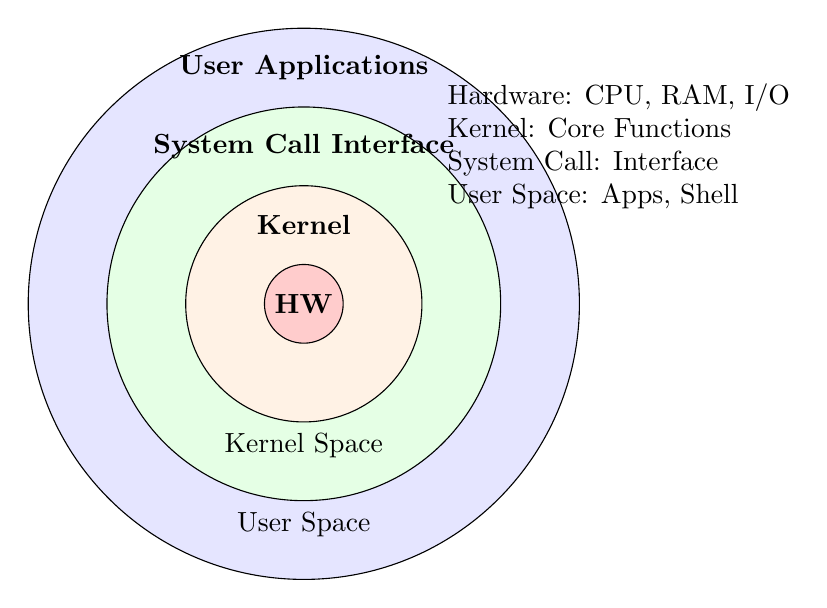
\begin{tikzpicture}
    % Concentric circles
    \draw [fill=blue!10] (0,0) circle (3.5cm);
    \node at (0,3) {\textbf{User Applications}};
    
    \draw [fill=green!10] (0,0) circle (2.5cm);
    \node at (0,2) {\textbf{System Call Interface}};
    
    \draw [fill=orange!10] (0,0) circle (1.5cm);
    \node at (0,1) {\textbf{Kernel}};
    
    \draw [fill=red!20] (0,0) circle (0.5cm);
    \node at (0,0) {\textbf{HW}};
    
    % Legend or labels
    \node [align=center] at (0,-2.8) {User Space};
    \node [align=center] at (0,-1.8) {Kernel Space};
    \node [align=left] at (4,2) {Hardware: CPU, RAM, I/O\\Kernel: Core Functions\\System Call: Interface\\User Space: Apps, Shell};
\end{tikzpicture}
\end{answerdiagram}


\begin{itemize}
    \item \textbf{User Space}: Applications and user programs
    \item \textbf{System Calls}: Interface between user and kernel
    \item \textbf{Kernel}: Core operating system functions
\end{itemize}

\begin{mnemonicbox}
\mnemonic{Users Use, Kernel Controls}
\end{mnemonicbox}
\end{solutionbox}

\questionmarks{2(b OR)}{4}{Explain Working of Search Engine.}

\begin{solutionbox}
\textbf{Answer:}

\textbf{Search Engine Working Process:}

\begin{answertable}{Search Engine Steps}
\begin{tabulary}{\linewidth}{|L|L|L|}
\hline
\textbf{Step} & \textbf{Process} & \textbf{Function} \\
\hline
\textbf{Crawling} & Web spiders scan websites & Discovers web pages \\
\hline
\textbf{Indexing} & Analyzes and stores content & Creates searchable database \\
\hline
\textbf{Ranking} & Applies algorithms & Determines relevance order \\
\hline
\textbf{Retrieval} & Returns results & Displays ranked results \\
\hline
\end{tabulary}
\end{answertable}

\begin{itemize}
    \item \textbf{Web Crawlers}: Automated bots scan internet content
    \item \textbf{Index Database}: Stores and organizes webpage information
    \item \textbf{Query Processing}: Analyzes user search terms
    \item \textbf{Result Ranking}: Uses algorithms to order results by relevance
\end{itemize}

\begin{mnemonicbox}
\mnemonic{Crawl, Index, Rank, Retrieve}
\end{mnemonicbox}
\end{solutionbox}

\questionmarks{2(c OR)}{7}{Difference between Open Source Software and Proprietary Software.}

\begin{solutionbox}
\textbf{Answer:}

\begin{answertable}{Open Source vs Proprietary Software}
\begin{tabulary}{\linewidth}{|L|L|L|}
\hline
\textbf{Aspect} & \textbf{Open Source Software} & \textbf{Proprietary Software} \\
\hline
\textbf{Source Code} & Freely available and modifiable & Closed and protected \\
\hline
\textbf{Cost} & Usually free & Requires license purchase \\
\hline
\textbf{Support} & Community-based & Vendor-provided \\
\hline
\textbf{Customization} & Fully customizable & Limited customization \\
\hline
\textbf{Examples} & Linux, Firefox, LibreOffice & Windows, MS Office, Photoshop \\
\hline
\textbf{Security} & Transparent, community-audited & Security through obscurity \\
\hline
\textbf{Updates} & Community-driven & Vendor-controlled \\
\hline
\end{tabulary}
\end{answertable}

\textbf{Key Differences:}
\begin{itemize}
    \item \textbf{Licensing}: Open source allows redistribution and modification
    \item \textbf{Cost Model}: Open source typically free vs. proprietary paid
    \item \textbf{Development}: Community collaboration vs. company-controlled
    \item \textbf{Transparency}: Open source code visible vs. proprietary hidden
\end{itemize}

\textbf{Advantages:}
\begin{itemize}
    \item \textbf{Open Source}: Cost-effective, customizable, secure
    \item \textbf{Proprietary}: Professional support, integrated features, user-friendly
\end{itemize}

\begin{mnemonicbox}
\mnemonic{Open Opens, Proprietary Protects}
\end{mnemonicbox}
\end{solutionbox}

\questionmarks{3(a)}{3}{Give full form of the following: OSI, LLC, FTP}

\begin{solutionbox}
\textbf{Answer:}

\textbf{Full Forms:}

\begin{answertable}{Abbreviations}
\begin{tabulary}{\linewidth}{|L|L|}
\hline
\textbf{Abbreviation} & \textbf{Full Form} \\
\hline
\textbf{OSI} & Open Systems Interconnection \\
\hline
\textbf{LLC} & Logical Link Control \\
\hline
\textbf{FTP} & File Transfer Protocol \\
\hline
\end{tabulary}
\end{answertable}

\begin{itemize}
    \item \textbf{OSI}: Networking reference model with 7 layers
    \item \textbf{LLC}: Sublayer of Data Link Layer in OSI model
    \item \textbf{FTP}: Protocol for transferring files over network
\end{itemize}

\begin{mnemonicbox}
\mnemonic{Open Logic Files}
\end{mnemonicbox}
\end{solutionbox}

\questionmarks{3(b)}{4}{Give advantages and disadvantages of Twisted Pair Cable.}

\begin{solutionbox}
\textbf{Answer:}

\textbf{Twisted Pair Cable Analysis:}

\begin{answertable}{Twisted Pair Pros and Cons}
\begin{tabulary}{\linewidth}{|L|L|}
\hline
\textbf{Advantages} & \textbf{Disadvantages} \\
\hline
\textbf{Low Cost} & \textbf{Limited Distance} \\
\hline
\textbf{Easy Installation} & \textbf{Electromagnetic Interference} \\
\hline
\textbf{Flexible} & \textbf{Lower Bandwidth} \\
\hline
\textbf{Widely Available} & \textbf{Security Issues} \\
\hline
\end{tabulary}
\end{answertable}

\textbf{Advantages:}
\begin{itemize}
    \item \textbf{Cost-effective}: Cheapest networking cable option
    \item \textbf{Easy Installation}: Simple to install and maintain
    \item \textbf{Flexibility}: Can be bent and routed easily
\end{itemize}

\textbf{Disadvantages:}
\begin{itemize}
    \item \textbf{Distance Limitation}: Maximum 100 meters without repeater
    \item \textbf{Interference}: Susceptible to electromagnetic interference
    \item \textbf{Bandwidth}: Lower data transmission rates compared to fiber
\end{itemize}

\begin{mnemonicbox}
\mnemonic{Twisted is Cheap but Limited}
\end{mnemonicbox}
\end{solutionbox}

\questionmarks{3(c)}{7}{What is Modulation? Explain Analog Modulation.}

\begin{solutionbox}
\textbf{Answer:}

\textbf{Modulation Definition:}
Process of varying carrier signal characteristics to transmit information over long distances.

\textbf{Analog Modulation Types:}

\begin{answertable}{Analog Modulation Types}
\begin{tabulary}{\linewidth}{|L|L|L|}
\hline
\textbf{Type} & \textbf{Parameter Varied} & \textbf{Application} \\
\hline
\textbf{AM} & Amplitude & Radio broadcasting \\
\hline
\textbf{FM} & Frequency & FM radio, TV sound \\
\hline
\textbf{PM} & Phase & Digital communications \\
\hline
\end{tabulary}
\end{answertable}

\textbf{Amplitude Modulation (AM):}

\begin{answerdiagram}{Amplitude Modulation}
\begin{tikzpicture}[auto, node distance=2cm]
    \node [gtu block] (modulator) {Modulator};
    \node [left=of modulator, yshift=1cm] (message) {Message Signal};
    \node [left=of modulator, yshift=-1cm] (carrier) {Carrier Signal};
    \node [right=of modulator] (output) {Modulated Signal};
    
    \draw [gtu arrow] (message) -| (modulator);
    \draw [gtu arrow] (carrier) -| (modulator);
    \draw [gtu arrow] (modulator) -- (output);
\end{tikzpicture}
\end{answerdiagram}

\textbf{Key Concepts:}
\begin{itemize}
    \item \textbf{Carrier Wave}: High-frequency signal for transmission
    \item \textbf{Message Signal}: Information to be transmitted
    \item \textbf{Modulation Index}: Degree of modulation applied
\end{itemize}

\textbf{Applications:}
\begin{itemize}
    \item \textbf{AM Radio}: 530-1710 kHz frequency band
    \item \textbf{FM Radio}: 88-108 MHz frequency band
    \item \textbf{Television}: Various modulation techniques
\end{itemize}

\textbf{Advantages:}
\begin{itemize}
    \item \textbf{Long Distance}: Enables long-range communication
    \item \textbf{Noise Immunity}: FM provides better noise resistance
\end{itemize}

\begin{mnemonicbox}
\mnemonic{Amplitude Alters, Frequency Fluctuates}
\end{mnemonicbox}
\end{solutionbox}

\questionmarks{3(a OR)}{3}{List out Network Topologies. Write Advantages and Disadvantages of Bus Topology.}

\begin{solutionbox}
\textbf{Answer:}

\textbf{Network Topologies:}
\begin{itemize}
    \item \textbf{Bus Topology}
    \item \textbf{Star Topology}
    \item \textbf{Ring Topology}
    \item \textbf{Mesh Topology}
    \item \textbf{Hybrid Topology}
\end{itemize}

\textbf{Bus Topology Analysis:}

\begin{answertable}{Bus Topology Pros and Cons}
\begin{tabulary}{\linewidth}{|L|L|}
\hline
\textbf{Advantages} & \textbf{Disadvantages} \\
\hline
\textbf{Simple Design} & \textbf{Single Point of Failure} \\
\hline
\textbf{Cost-effective} & \textbf{Limited Cable Length} \\
\hline
\textbf{Easy to Expand} & \textbf{Performance Degradation} \\
\hline
\end{tabulary}
\end{answertable}

\begin{mnemonicbox}
\mnemonic{Bus is Simple but Single-failure-prone}
\end{mnemonicbox}
\end{solutionbox}

\questionmarks{3(b OR)}{4}{Differentiate Serial and Parallel Transmission.}

\begin{solutionbox}
\textbf{Answer:}

\begin{answertable}{Serial vs Parallel Transmission}
\begin{tabulary}{\linewidth}{|L|L|L|}
\hline
\textbf{Aspect} & \textbf{Serial Transmission} & \textbf{Parallel Transmission} \\
\hline
\textbf{Data Path} & Single communication line & Multiple lines simultaneously \\
\hline
\textbf{Speed} & Slower for short distances & Faster for short distances \\
\hline
\textbf{Cost} & Lower cost & Higher cost \\
\hline
\textbf{Distance} & Suitable for long distances & Limited to short distances \\
\hline
\end{tabulary}
\end{answertable}

\textbf{Characteristics:}
\begin{itemize}
    \item \textbf{Serial}: Bits transmitted one after another
    \item \textbf{Parallel}: Multiple bits transmitted simultaneously
    \item \textbf{Applications}: Serial for networks, Parallel for internal buses
\end{itemize}

\begin{mnemonicbox}
\mnemonic{Serial Single-file, Parallel Processes}
\end{mnemonicbox}
\end{solutionbox}

\questionmarks{3(c OR)}{7}{Explain Transmission Modes.}

\begin{solutionbox}
\textbf{Answer:}

\textbf{Transmission Modes Classification:}

\begin{answertable}{Transmission Modes}
\begin{tabulary}{\linewidth}{|L|L|L|L|}
\hline
\textbf{Mode} & \textbf{Direction} & \textbf{Examples} & \textbf{Applications} \\
\hline
\textbf{Simplex} & One-way only & Radio, TV broadcast & Broadcasting \\
\hline
\textbf{Half-duplex} & Two-way, not simultaneous & Walkie-talkie & Turn-based communication \\
\hline
\textbf{Full-duplex} & Two-way simultaneous & Telephone & Real-time communication \\
\hline
\end{tabulary}
\end{answertable}

\textbf{Detailed Explanation:}

\textbf{1. Simplex Mode:}
\begin{itemize}
    \item \textbf{Unidirectional}: Data flows in one direction only
    \item \textbf{Examples}: Television broadcasting, radio transmission
    \item \textbf{Advantage}: Simple implementation
    \item \textbf{Disadvantage}: No feedback possible
\end{itemize}

\textbf{2. Half-duplex Mode:}
\begin{itemize}
    \item \textbf{Bidirectional}: Data can flow both ways, but not simultaneously
    \item \textbf{Examples}: Walkie-talkies, CB radio
    \item \textbf{Advantage}: Two-way communication with single channel
    \item \textbf{Disadvantage}: Cannot send and receive simultaneously
\end{itemize}

\textbf{3. Full-duplex Mode:}
\begin{itemize}
    \item \textbf{Simultaneous Bidirectional}: Data flows both ways at same time
    \item \textbf{Examples}: Telephone conversations, modern networks
    \item \textbf{Advantage}: Efficient real-time communication
    \item \textbf{Disadvantage}: Requires more complex implementation
\end{itemize}

\begin{mnemonicbox}
\mnemonic{Simplex Single, Half-duplex Halts, Full-duplex Flows}
\end{mnemonicbox}
\end{solutionbox}

\questionmarks{4(a)}{3}{Draw Crossover Ethernet Cable.}

\begin{solutionbox}
\textbf{Answer:}

\textbf{Crossover Cable Wiring Diagram:}

\begin{answerdiagram}{Crossover Cable Wiring}
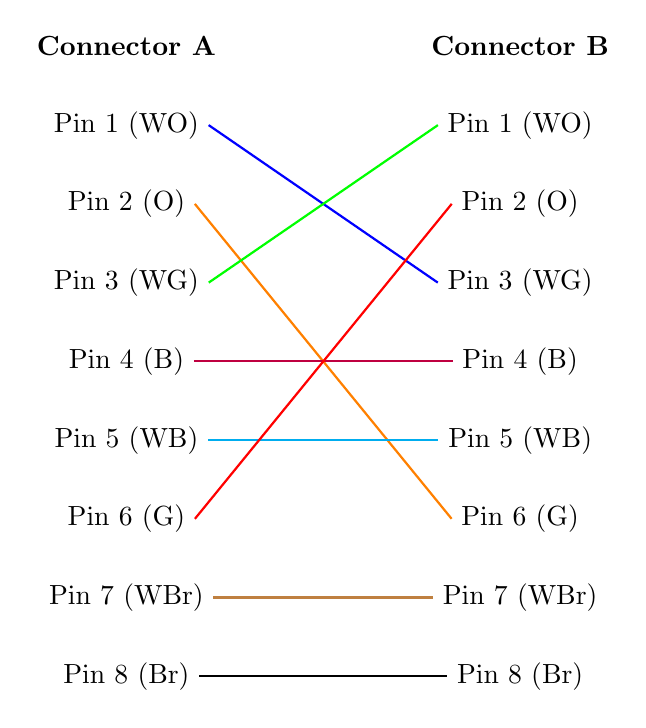
\begin{tikzpicture}
    % RJ-45 Connector A
    \node (A1) at (0,7) {Pin 1 (WO)};
    \node (A2) at (0,6) {Pin 2 (O)};
    \node (A3) at (0,5) {Pin 3 (WG)};
    \node (A4) at (0,4) {Pin 4 (B)};
    \node (A5) at (0,3) {Pin 5 (WB)};
    \node (A6) at (0,2) {Pin 6 (G)};
    \node (A7) at (0,1) {Pin 7 (WBr)};
    \node (A8) at (0,0) {Pin 8 (Br)};
    
    \node at (0,8) {\textbf{Connector A}};

    % RJ-45 Connector B
    \node (B1) at (5,7) {Pin 1 (WO)};
    \node (B2) at (5,6) {Pin 2 (O)};
    \node (B3) at (5,5) {Pin 3 (WG)};
    \node (B4) at (5,4) {Pin 4 (B)};
    \node (B5) at (5,3) {Pin 5 (WB)};
    \node (B6) at (5,2) {Pin 6 (G)};
    \node (B7) at (5,1) {Pin 7 (WBr)};
    \node (B8) at (5,0) {Pin 8 (Br)};
    
    \node at (5,8) {\textbf{Connector B}};
    
    % Connections for Crossover (1-3, 2-6, 3-1, 6-2)
    \draw [thick, blue] (A1.east) -- (B3.west);
    \draw [thick, orange] (A2.east) -- (B6.west);
    \draw [thick, green] (A3.east) -- (B1.west);
    \draw [thick, purple] (A4.east) -- (B4.west);
    \draw [thick, cyan] (A5.east) -- (B5.west);
    \draw [thick, red] (A6.east) -- (B2.west);
    \draw [thick, brown] (A7.east) -- (B7.west);
    \draw [thick, black] (A8.east) -- (B8.west);
\end{tikzpicture}
\end{answerdiagram}

\textbf{Key Points:}
\begin{itemize}
    \item \textbf{Purpose}: Direct connection between similar devices
    \item \textbf{Crossed Pairs}: Transmit and receive pairs are swapped
    \item \textbf{Usage}: PC to PC, Switch to Switch connections
\end{itemize}

\begin{mnemonicbox}
\mnemonic{Cross Connects Computers}
\end{mnemonicbox}
\end{solutionbox}

\questionmarks{4(b)}{4}{Difference between IPv4 and IPv6.}

\begin{solutionbox}
\textbf{Answer:}

\begin{answertable}{IPv4 vs IPv6}
\begin{tabulary}{\linewidth}{|L|L|L|}
\hline
\textbf{Feature} & \textbf{IPv4} & \textbf{IPv6} \\
\hline
\textbf{Address Size} & 32 bits & 128 bits \\
\hline
\textbf{Address Format} & Dotted decimal & Hexadecimal colon \\
\hline
\textbf{Address Space} & 4.3 billion addresses & 340 undecillion addresses \\
\hline
\textbf{Header Size} & Variable (20-60 bytes) & Fixed (40 bytes) \\
\hline
\end{tabulary}
\end{answertable}

\textbf{Key Differences:}
\begin{itemize}
    \item \textbf{IPv4 Example}: 192.168.1.1
    \item \textbf{IPv6 Example}: 2001:0db8:85a3:0000:0000:8a2e:0370:7334
    \item \textbf{Security}: IPv6 has built-in IPSec support
    \item \textbf{NAT}: IPv4 requires NAT, IPv6 eliminates need
\end{itemize}

\begin{mnemonicbox}
\mnemonic{IPv4 Four-billion, IPv6 Six-teen-times-more}
\end{mnemonicbox}
\end{solutionbox}

\questionmarks{4(c)}{7}{Draw neat and clean figure of OSI Model and write down the functionality of Physical Layer and Data Link Layer.}

\begin{solutionbox}
\textbf{Answer:}

\textbf{OSI Model Diagram:}

\begin{answerdiagram}{OSI Model}
\begin{tikzpicture}[gtu tree]
    % Simple stack
    \node [gtu block] (app) at (0,6) {Application Layer (7)};
    \node [gtu block] (pres) at (0,5) {Presentation Layer (6)};
    \node [gtu block] (sess) at (0,4) {Session Layer (5)};
    \node [gtu block] (trans) at (0,3) {Transport Layer (4)};
    \node [gtu block] (net) at (0,2) {Network Layer (3)};
    \node [gtu block] (data) at (0,1) {Data Link Layer (2)};
    \node [gtu block] (phys) at (0,0) {Physical Layer (1)};
    
    \draw [->] (app) -- (pres);
    \draw [->] (pres) -- (sess);
    \draw [->] (sess) -- (trans);
    \draw [->] (trans) -- (net);
    \draw [->] (net) -- (data);
    \draw [->] (data) -- (phys);
\end{tikzpicture}
\end{answerdiagram}

\textbf{Layer Functions:}

\begin{answertable}{Top Two Layers Functions}
\begin{tabulary}{\linewidth}{|L|L|L|}
\hline
\textbf{Layer} & \textbf{Function} & \textbf{Examples} \\
\hline
\textbf{Physical (Layer 1)} & Bit transmission over medium & Cables, hubs, repeaters \\
\hline
\textbf{Data Link (Layer 2)} & Frame delivery between adjacent nodes & Switches, MAC addresses \\
\hline
\end{tabulary}
\end{answertable}

\textbf{Physical Layer Functions:}
\begin{itemize}
    \item \textbf{Bit Transmission}: Converts data into electrical/optical signals
    \item \textbf{Medium Specification}: Defines cable types and connectors
    \item \textbf{Signal Encoding}: Determines how bits are represented
    \item \textbf{Transmission Rate}: Controls data speed
\end{itemize}

\textbf{Data Link Layer Functions:}
\begin{itemize}
    \item \textbf{Frame Formation}: Organizes bits into frames
    \item \textbf{Error Detection}: Identifies transmission errors
    \item \textbf{Flow Control}: Manages data transmission rate
    \item \textbf{MAC Addressing}: Uses hardware addresses for local delivery
\end{itemize}

\begin{mnemonicbox}
\mnemonic{Physical Pushes, Data-Link Delivers}
\end{mnemonicbox}
\end{solutionbox}

\questionmarks{4(a OR)}{3}{Explain Time Division Multiplexing.}

\begin{solutionbox}
\textbf{Answer:}

\textbf{Time Division Multiplexing (TDM):}

\begin{answerdiagram}{TDM Time Slots}
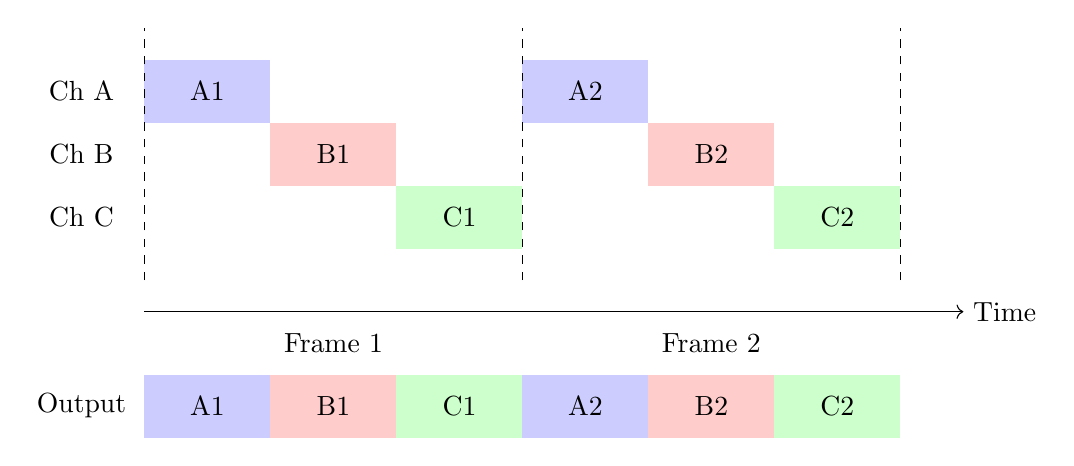
\begin{tikzpicture}[scale=0.8]
    % Channel A
    \fill [blue!20] (0,2) rectangle (2,3); \node at (1,2.5) {A1};
    \fill [blue!20] (6,2) rectangle (8,3); \node at (7,2.5) {A2};
    \node at (-1, 2.5) {Ch A};

    % Channel B
    \fill [red!20] (2,1) rectangle (4,2); \node at (3,1.5) {B1};
    \fill [red!20] (8,1) rectangle (10,2); \node at (9,1.5) {B2};
    \node at (-1, 1.5) {Ch B};
    
    % Channel C
    \fill [green!20] (4,0) rectangle (6,1); \node at (5,0.5) {C1};
    \fill [green!20] (10,0) rectangle (12,1); \node at (11,0.5) {C2};
    \node at (-1, 0.5) {Ch C};
    
    % Draw timeline/frames
    \draw [->] (0,-1) -- (13,-1) node[right] {Time};
    
    % Frame 1
    \draw [dashed] (0,-0.5) -- (0,3.5);
    \draw [dashed] (6,-0.5) -- (6,3.5);
    \node at (3,-1.5) {Frame 1};
    
    % Frame 2
    \draw [dashed] (12,-0.5) -- (12,3.5);
    \node at (9,-1.5) {Frame 2};
    
    % Multiplexed Output Stream
    \fill [blue!20] (0,-3) rectangle (2,-2); \node at (1,-2.5) {A1};
    \fill [red!20] (2,-3) rectangle (4,-2); \node at (3,-2.5) {B1};
    \fill [green!20] (4,-3) rectangle (6,-2); \node at (5,-2.5) {C1};
    \fill [blue!20] (6,-3) rectangle (8,-2); \node at (7,-2.5) {A2};
    \fill [red!20] (8,-3) rectangle (10,-2); \node at (9,-2.5) {B2};
    \fill [green!20] (10,-3) rectangle (12,-2); \node at (11,-2.5) {C2};
    \node at (-1, -2.5) {Output};
    
\end{tikzpicture}
\end{answerdiagram}

\textbf{TDM Characteristics:}
\begin{itemize}
    \item \textbf{Time Slots}: Each channel gets dedicated time period
    \item \textbf{Synchronization}: All channels must be synchronized
    \item \textbf{Bandwidth Sharing}: Single high-speed link shared among multiple channels
\end{itemize}

\begin{mnemonicbox}
\mnemonic{Time Takes Turns}
\end{mnemonicbox}
\end{solutionbox}

\questionmarks{4(b OR)}{4}{List out types of Networking Device and Explain any one.}

\begin{solutionbox}
\textbf{Answer:}

\textbf{Networking Devices:}

\begin{answertable}{Network Devices}
\begin{tabulary}{\linewidth}{|L|L|L|}
\hline
\textbf{Device} & \textbf{Layer} & \textbf{Function} \\
\hline
\textbf{Hub} & Physical & Signal repeater \\
\hline
\textbf{Switch} & Data Link & Frame switching \\
\hline
\textbf{Router} & Network & Packet routing \\
\hline
\textbf{Bridge} & Data Link & Network segmentation \\
\hline
\end{tabulary}
\end{answertable}

\textbf{Switch Explanation:}
\begin{itemize}
    \item \textbf{Function}: Forwards frames based on MAC addresses
    \item \textbf{Learning}: Builds MAC address table dynamically
    \item \textbf{Collision Domain}: Each port creates separate collision domain
    \item \textbf{Full-duplex}: Simultaneous send/receive on each port
\end{itemize}

\textbf{Advantages:}
\begin{itemize}
    \item \textbf{Bandwidth}: Full bandwidth per port
    \item \textbf{Security}: Frames sent only to intended recipient
    \item \textbf{Collision}: Eliminates collisions
\end{itemize}

\begin{mnemonicbox}
\mnemonic{Switch Smartly Sends}
\end{mnemonicbox}
\end{solutionbox}

\questionmarks{4(c OR)}{7}{What is Computer Network? Explain types of Computer Network.}

\begin{solutionbox}
\textbf{Answer:}

\textbf{Computer Network Definition:}
Interconnected collection of autonomous computers that can communicate and share resources.

\textbf{Types of Computer Networks:}

\begin{answertable}{Network Types}
\begin{tabulary}{\linewidth}{|L|L|L|L|}
\hline
\textbf{Type} & \textbf{Coverage} & \textbf{Examples} & \textbf{Characteristics} \\
\hline
\textbf{LAN} & Local area (building) & Office network & High speed, low cost \\
\hline
\textbf{MAN} & Metropolitan area (city) & City-wide network & Medium speed, moderate cost \\
\hline
\textbf{WAN} & Wide area (country/world) & Internet & Lower speed, high cost \\
\hline
\end{tabulary}
\end{answertable}

\textbf{Detailed Explanation:}

\textbf{1. Local Area Network (LAN):}
\begin{itemize}
    \item \textbf{Coverage}: Single building or campus
    \item \textbf{Speed}: High (100 Mbps to 10 Gbps)
    \item \textbf{Technology}: Ethernet, Wi-Fi
    \item \textbf{Ownership}: Single organization
\end{itemize}

\textbf{2. Metropolitan Area Network (MAN):}
\begin{itemize}
    \item \textbf{Coverage}: City or metropolitan area
    \item \textbf{Speed}: Medium (10-100 Mbps)
    \item \textbf{Technology}: Fiber optic, microwave
    \item \textbf{Examples}: Cable TV networks
\end{itemize}

\textbf{3. Wide Area Network (WAN):}
\begin{itemize}
    \item \textbf{Coverage}: Countries or continents
    \item \textbf{Speed}: Variable (depends on technology)
    \item \textbf{Technology}: Satellite, leased lines
    \item \textbf{Examples}: Internet, corporate networks
\end{itemize}

\textbf{Network Benefits:}
\begin{itemize}
    \item \textbf{Resource Sharing}: Files, printers, applications
    \item \textbf{Communication}: Email, messaging, video conferencing
    \item \textbf{Cost Reduction}: Shared resources reduce costs
    \item \textbf{Data Backup}: Centralized backup systems
\end{itemize}

\begin{mnemonicbox}
\mnemonic{Local Loves, Metro Manages, Wide Wanders}
\end{mnemonicbox}
\end{solutionbox}

\questionmarks{5(a)}{3}{Explain the need for information security.}

\begin{solutionbox}
\textbf{Answer:}

\textbf{Information Security Needs:}

\begin{answertable}{Security Needs}
\begin{tabulary}{\linewidth}{|L|L|L|}
\hline
\textbf{Threat} & \textbf{Impact} & \textbf{Protection Need} \\
\hline
\textbf{Data Theft} & Financial loss & Confidentiality \\
\hline
\textbf{Unauthorized Access} & Privacy breach & Access control \\
\hline
\textbf{System Attacks} & Service disruption & Availability \\
\hline
\end{tabulary}
\end{answertable}

\textbf{Key Requirements:}
\begin{itemize}
    \item \textbf{Confidentiality}: Protecting sensitive information from unauthorized access
    \item \textbf{Data Protection}: Preventing loss or corruption of valuable data
    \item \textbf{Business Continuity}: Ensuring systems remain operational
\end{itemize}

\begin{mnemonicbox}
\mnemonic{Security Secures Sensitive Systems}
\end{mnemonicbox}
\end{solutionbox}

\questionmarks{5(b)}{4}{Write advantages and disadvantages of Fiber Optic Cable.}

\begin{solutionbox}
\textbf{Answer:}

\begin{answertable}{Fiber Optic Pros and Cons}
\begin{tabulary}{\linewidth}{|L|L|}
\hline
\textbf{Advantages} & \textbf{Disadvantages} \\
\hline
\textbf{High Bandwidth} & \textbf{High Cost} \\
\hline
\textbf{Immunity to EMI} & \textbf{Difficult Installation} \\
\hline
\textbf{Long Distance} & \textbf{Fragile Nature} \\
\hline
\textbf{Secure Transmission} & \textbf{Specialized Equipment} \\
\hline
\end{tabulary}
\end{answertable}

\textbf{Advantages:}
\begin{itemize}
    \item \textbf{Speed}: Highest data transmission rates
    \item \textbf{Distance}: Can span long distances without signal degradation
    \item \textbf{Security}: Difficult to tap, providing secure communication
\end{itemize}

\textbf{Disadvantages:}
\begin{itemize}
    \item \textbf{Cost}: Expensive cable and equipment
    \item \textbf{Installation}: Requires skilled technicians
    \item \textbf{Maintenance}: Difficult to repair and splice
\end{itemize}

\begin{mnemonicbox}
\mnemonic{Fiber is Fast but Fragile}
\end{mnemonicbox}
\end{solutionbox}

\questionmarks{5(c)}{7}{List out types of Attack. And Explain any two web based attack.}

\begin{solutionbox}
\textbf{Answer:}

\textbf{Types of Attacks:}

\begin{answertable}{Attack Categories}
\begin{tabulary}{\linewidth}{|L|L|L|}
\hline
\textbf{Category} & \textbf{Attack Types} & \textbf{Target} \\
\hline
\textbf{Web-based} & SQL Injection, XSS, CSRF & Web applications \\
\hline
\textbf{Network} & DoS, DDoS, Man-in-Middle & Network infrastructure \\
\hline
\textbf{Malware} & Virus, Trojan, Ransomware & Systems and data \\
\hline
\textbf{Social} & Phishing, Social Engineering & Human users \\
\hline
\end{tabulary}
\end{answertable}

\textbf{Web-based Attacks Explained:}

\textbf{1. SQL Injection:}
\begin{itemize}
    \item \textbf{Method}: Inserting malicious SQL code into web application inputs
    \item \textbf{Impact}: Unauthorized database access, data theft
    \item \textbf{Example}: Entering \code{'; DROP TABLE users;--} in login form
    \item \textbf{Prevention}: Input validation, parameterized queries
    \item \textbf{Severity}: Can compromise entire database
\end{itemize}

\textbf{2. Cross-Site Scripting (XSS):}
\begin{itemize}
    \item \textbf{Method}: Injecting malicious scripts into web pages
    \item \textbf{Impact}: Session hijacking, cookie theft, page defacement
    \item \textbf{Types}: Stored XSS, Reflected XSS, DOM-based XSS
    \item \textbf{Prevention}: Input sanitization, output encoding
    \item \textbf{Target}: Affects users visiting compromised websites
\end{itemize}

\begin{mnemonicbox}
\mnemonic{SQL Steals, XSS eXploits Scripts}
\end{mnemonicbox}
\end{solutionbox}

\questionmarks{5(a OR)}{3}{Explain Confidentiality, Integrity and Availability.}

\begin{solutionbox}
\textbf{Answer:}

\textbf{CIA Triad Components:}

\begin{answertable}{CIA Triad}
\begin{tabulary}{\linewidth}{|L|L|L|}
\hline
\textbf{Component} & \textbf{Definition} & \textbf{Examples} \\
\hline
\textbf{Confidentiality} & Information access only by authorized users & Encryption, access controls \\
\hline
\textbf{Integrity} & Data accuracy and completeness & Checksums, digital signatures \\
\hline
\textbf{Availability} & Systems accessible when needed & Redundancy, backup systems \\
\hline
\end{tabulary}
\end{answertable}

\textbf{Key Concepts:}
\begin{itemize}
    \item \textbf{Confidentiality}: Keeps information secret from unauthorized users
    \item \textbf{Integrity}: Ensures data hasn't been modified without authorization
    \item \textbf{Availability}: Guarantees systems are operational when required
\end{itemize}

\begin{mnemonicbox}
\mnemonic{CIA Completely Protects Information}
\end{mnemonicbox}
\end{solutionbox}

\questionmarks{5(b OR)}{4}{Find class of following IP addresses.}

\begin{solutionbox}
\textbf{Answer:}

\textbf{IP Address Class Identification:}

\begin{answertable}{IP Class Finder}
\begin{tabulary}{\linewidth}{|L|L|L|L|}
\hline
\textbf{IP Address} & \textbf{First Octet} & \textbf{Class} & \textbf{Range} \\
\hline
\textbf{192.12.44.12} & 192 & Class C & 192-223 \\
\hline
\textbf{123.77.42.213} & 123 & Class A & 1-126 \\
\hline
\textbf{190.65.22.15} & 190 & Class B & 128-191 \\
\hline
\textbf{10.0.0.11} & 10 & Class A (Private) & 1-126 \\
\hline
\end{tabulary}
\end{answertable}

\textbf{Class Characteristics:}
\begin{itemize}
    \item \textbf{Class A}: 1-126 (first bit 0), supports large networks
    \item \textbf{Class B}: 128-191 (first two bits 10), medium networks
    \item \textbf{Class C}: 192-223 (first three bits 110), small networks
    \item \textbf{Private IPs}: 10.x.x.x, 172.16-31.x.x, 192.168.x.x
\end{itemize}

\begin{mnemonicbox}
\mnemonic{A is Awesome, B is Better, C is Compact}
\end{mnemonicbox}
\end{solutionbox}

\questionmarks{5(c OR)}{7}{Explain Cryptography.}

\begin{solutionbox}
\textbf{Answer:}

\textbf{Cryptography Definition:}
Science of securing communication through encoding information so only authorized parties can access it.

\textbf{Cryptography Types:}

\begin{answertable}{Crypto Types}
\begin{tabulary}{\linewidth}{|L|L|L|L|}
\hline
\textbf{Type} & \textbf{Key Usage} & \textbf{Examples} & \textbf{Applications} \\
\hline
\textbf{Symmetric} & Single shared key & DES, AES & Fast bulk encryption \\
\hline
\textbf{Asymmetric} & Public-private key pair & RSA, ECC & Digital signatures, key exchange \\
\hline
\textbf{Hash Functions} & One-way transformation & MD5, SHA & Data integrity, passwords \\
\hline
\end{tabulary}
\end{answertable}

\textbf{Cryptographic Process:}

\begin{answerdiagram}{Cryptography Flow}
\begin{tikzpicture}[auto, node distance=2cm]
    \node [gtu block] (plain) {Plaintext};
    \node [gtu block, right=of plain] (encrypt) {Encryption};
    \node [gtu block, right=of encrypt] (cipher) {Ciphertext};
    \node [gtu block, right=of cipher] (decrypt) {Decryption};
    \node [gtu block, right=of decrypt] (plain2) {Plaintext};
    
    \node [gtu block, above=of encrypt] (key) {Key};
    
    \draw [gtu arrow] (plain) -- (encrypt);
    \draw [gtu arrow] (encrypt) -- (cipher);
    \draw [gtu arrow] (cipher) -- (decrypt);
    \draw [gtu arrow] (decrypt) -- (plain2);
    
    \draw [gtu arrow] (key) -- (encrypt);
    \draw [gtu arrow] (key) -| (decrypt);
\end{tikzpicture}
\end{answerdiagram}

\textbf{Detailed Explanation:}

\textbf{1. Symmetric Cryptography:}
\begin{itemize}
    \item \textbf{Single Key}: Same key for encryption and decryption
    \item \textbf{Speed}: Fast processing for large amounts of data
    \item \textbf{Challenge}: Secure key distribution
\end{itemize}

\textbf{2. Asymmetric Cryptography:}
\begin{itemize}
    \item \textbf{Key Pairs}: Public key (shareable) and private key (secret)
    \item \textbf{Digital Signatures}: Proves authenticity and non-repudiation
\end{itemize}

\begin{mnemonicbox}
\mnemonic{Cryptography Creates Coded Communications}
\end{mnemonicbox}
\end{solutionbox}

\end{document}
